\section*{Aufgabe 3 (30 Punkte)}
\vspace{0.4cm}
\subsection*{\frage{1}{4}}
Es sei
\begin{align*}
	s = \sum \limits_{i= 1}^3
	\sum \limits_{j= 1}^2
	\sum \limits_{k= 1}^4
	(i + jk).
\end{align*}
Dann gilt:
\renewcommand{\labelenumi}{(\alph{enumi})}
\begin{enumerate}
	\item 
	$ s= 138 $.
	\item
	$ s= 144 $.
	\item
	$ s= 132 $.
	\item
	$ s= 180 $.
	\item
	$ s= 120 $.
	\item
	$ s= 128 $.
\end{enumerate}
\ \\
\textbf{Lösung:}
\begin{mdframed}
\underline{\textbf{Vorgehensweise:}}
\renewcommand{\labelenumi}{\theenumi.}
\begin{enumerate}
\item Löse die Summe auf.
\end{enumerate}
\end{mdframed}

\underline{1. Löse die Summe auf}\\
Wir lösen die Summe durch Umformungen auf:
\begin{align*}
	s 
	&= 
	\sum \limits_{i= 1}^3
	\sum \limits_{j= 1}^2
	\sum \limits_{k= 1}^4
	(i + jk)
	=
	\sum \limits_{i= 1}^3
	\left(
	\sum \limits_{j= 1}^2
	\sum \limits_{k= 1}^4
	i 
	+ 
	\sum \limits_{j= 1}^2
	\sum \limits_{k= 1}^4
	jk
	\right)
		=
	\sum \limits_{i= 1}^3
	\left(
	8
	\cdot i
	+ 
	\sum \limits_{k= 1}^4
	k
	+ 
	2 \cdot \sum \limits_{k= 1}^4
	k
	\right)\\
	&=
	\sum \limits_{i= 1}^3
	\left(
	8
	\cdot i
	+ 
	10
	+ 
	20
	\right)
	=
	8  \cdot \sum \limits_{i= 1}^3 i + 3 \cdot 30
	=
	8 \cdot 6 + 90 = 48 + 90 \\
	&= 138.
\end{align*}
Damit ist die Antwort (a) korrekt.

\newpage

\subsection*{\frage{2}{4}}
Der Grenzwert
\begin{align*}
	\lim\limits_{x \to 0 }
	\frac{\sqrt[n]{a+x} - \sqrt[n]{a-x}}{x}
\end{align*}
für einen fest gewählten Parameter $ a > 0  $ ist gleich:
\renewcommand{\labelenumi}{(\alph{enumi})}
\begin{enumerate}
	\item 
	$0$.
	\item
	$1$.
	\item
	$\frac{\sqrt[n]{a}}{na}$.
	\item
	$\frac{2}{n} \sqrt[n]{a}$.
	\item
	$\frac{2}{n} \sqrt[n]{a^{1-n}}$.
	\item
	Der obige Ausdruck hat für $ x \to 0 $ keinen Grenzwert.	
\end{enumerate}
\ \\
\textbf{Lösung:}
\begin{mdframed}
\underline{\textbf{Vorgehensweise:}}
\renewcommand{\labelenumi}{\theenumi.}
\begin{enumerate}
\item Wende die Regel von l'H\^{o}pital an
\end{enumerate}
\end{mdframed}

\underline{1. Wende die Regel von l'H\^{o}pital an}\\
Wegen
\begin{align*}
	\lim \limits_{x \to 0} \sqrt[n]{a+x} - \sqrt[n]{a-x} = 0
	\ \textrm{und} \
	\lim \limits_{x \to 0} x = 0
\end{align*}
liegt der l'H\^{o}pital-Fall \glqq$ \nicefrac{0}{0} $\grqq~vor.
Zunächst bestimmen wir die Ableitung des Zählers:
\begin{align*}
	\frac{\mathrm{d}}{ \mathrm{dx} }\sqrt[n]{a+x}
	&=
	\frac{\mathrm{d}}{\mathrm{dx} }(a+x)^{\frac{1}{n}}
	=
	\frac{1}{n}(a+x)^{\frac{1}{n} -1}
	= 
	\frac{1}{n}(a+x)^{\left(1 - n\right) \frac{1}{n} }
	=
	\sqrt[n]{(a+x)^{1 - n }}\\
	\frac{\mathrm{d}}{\mathrm{dx} }\sqrt[n]{a-x}
	&=
	\frac{\mathrm{d}}{\mathrm{dx} }(a-x)^{\frac{1}{n}}
	=
	...
	=
	-\frac{1}{n}\sqrt[n]{(a-x)^{1 - n }}.
\end{align*}
Damit ergibt sich für die Ableitung des Zählers:
\begin{align*}
		\frac{\mathrm{d}}{ \mathrm{dx} } \left(\sqrt[n]{a+x} - \sqrt[n]{a-x} \right)
		&=
		\frac{1}{n}\sqrt[n]{(a+x)^{1 - n }} -\left(-\frac{1}{n}\sqrt[n]{(a-x)^{1 - n }}\right)
		=
		\frac{1}{n}\sqrt[n]{(a+x)^{1 - n }} +\frac{1}{n}\sqrt[n]{(a-x)^{1 - n }}\\
		&=
		\frac{1}{n}
		\left(\sqrt[n]{(a+x)^{1 - n }}+\sqrt[n]{(a-x)^{1 - n }}\right).
\end{align*}
Mit der Regel von l'H\^{o}pital erhalten wir dann:
\begin{align*}
	\lim \limits_{x \to 0}
	\frac{\sqrt[n]{a+x} - \sqrt[n]{a-x}}{x}
	&=
	\lim \limits_{x \to 0}
	\frac{\frac{\mathrm{d}}{ \mathrm{dx} } \left(\sqrt[n]{a+x} - \sqrt[n]{a-x} \right)}{ \frac{\mathrm{d}}{ \mathrm{dx} }  x}
	=
	\lim \limits_{x \to 0}
	\frac{\frac{1}{n}
		\left(\sqrt[n]{(a+x)^{1 - n }}+\sqrt[n]{(a-x)^{1 - n }}\right)}{1}\\
	&=\frac{1}{n}\cdot
	\left(\sqrt[n]{a^{1 - n }} + \sqrt[n]{a^{1 - n }}\right)
	=
	\frac{2}{n} \cdot \sqrt[n]{a^{1 - n }}
\end{align*}



\newpage
\subsection*{\frage{3}{4}}
Gegeben ist die Funktion
\begin{align*}
	f(x) = x^{\ln(x)}.
\end{align*}
Welcher der folgenden Ausdrücke beschreibt die erste Ableitung von $ f $ ?
\renewcommand{\labelenumi}{(\alph{enumi})}
\begin{enumerate}
	\item 
	$ f^\prime(x) = [\ln(x)]^2 x^{\ln(x)} \frac{1}{x}$.
	\item
	$ f^\prime(x) =2 x^{\ln(x) -1} \ln(x) $.
	\item
	$ f^\prime(x) = \ln(x) x^{\ln(x) -1} $.
	\item
	$ f^\prime(x) =  x^{\ln(x) }\ln(x)\frac{1}{x} $.
	\item
	Keine der vorangehenden Formeln für $ f^\prime(x)  $ ist korrekt.
\end{enumerate}
\ \\
\textbf{Lösung:}
\begin{mdframed}
\underline{\textbf{Vorgehensweise:}}
\renewcommand{\labelenumi}{\theenumi.}
\begin{enumerate}
\item 
\end{enumerate}
\end{mdframed}
%\allowdisplaybreaks
\underline{1. }\\


\newpage
\subsection*{\frage{4}{4}}
Gegeben ist die Funktion $ f $ zweier reeller Variablen
\begin{align*}
	f \ : \ D_f \to \R, \ (x,y) \mapsto z = f(x,y) =\sqrt{(36 - x^2 -y^2) y}.
\end{align*}
Welches der folgenden Bilder zeigt grau schraffiert den Definitionsbereich $ D_f \subset \R^2 $ von $ f $?
\renewcommand{\labelenumi}{(\alph{enumi})}
\begin{enumerate}
	\item 
	\begin{center}
		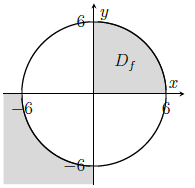
\includegraphics[scale=0.6]{pictures/3_4_a}
	\end{center}
	\item 
	\begin{center}
		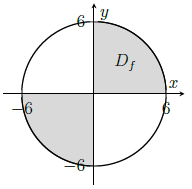
\includegraphics[scale=0.6]{pictures/3_4_b}
	\end{center}
	\item
	\begin{center}
		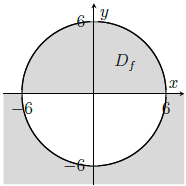
\includegraphics[scale=0.6]{pictures/3_4_c}
	\end{center}
	\item
	\begin{center}
		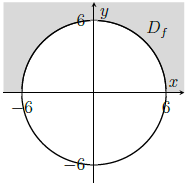
\includegraphics[scale=0.6]{pictures/3_4_d}
	\end{center}
\end{enumerate}
\ \\
\textbf{Lösung:}
\begin{mdframed}
\underline{\textbf{Vorgehensweise:}}
\renewcommand{\labelenumi}{\theenumi.}
\begin{enumerate}
\item .

\end{enumerate}
\end{mdframed}

\underline{1.}\\

\newpage

\subsection*{\frage{5}{3}}
Welche der folgenden Funktionen gehört zur unten dargestellten Fläche?\\
\begin{center}
	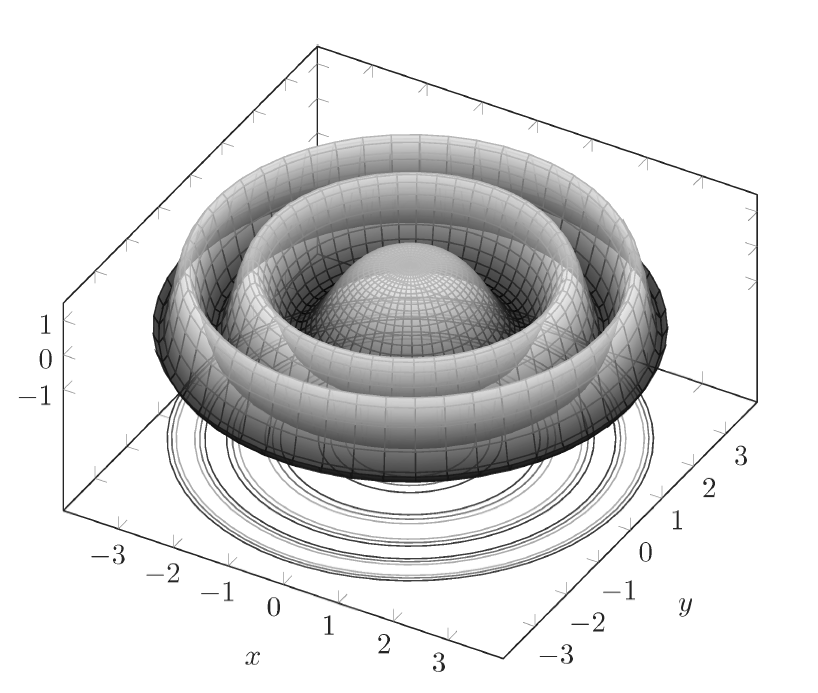
\includegraphics[scale=0.5]{pictures/3_5}
\end{center}
\renewcommand{\labelenumi}{(\alph{enumi})}
\begin{enumerate}
	\item 
	$ z = f_1(x,y) = e^{-(x+y^2)} $.
	\item
	$ z = f_2(x,y) = e^{x} e^y $.
	\item
	$ z = f_3(x,y) = e^{2 -x^2 +y^2}  $.
	\item
	$ z = f_4(x,y) = \cos(x^2 +y^2) $.
	\item
	$ z = f_5(x,y) = 2^{-(x + y^2)} $.
	\item
	$ z = f_6(x,y) = \sin(x+y) $.
\end{enumerate}
\ \\
\textbf{Lösung:}
\begin{mdframed}
\underline{\textbf{Vorgehensweise:}}
\renewcommand{\labelenumi}{\theenumi.}
\begin{enumerate}
\item .
\end{enumerate}
\end{mdframed}

\underline{1. }\\

\newpage

\subsection*{\frage{6}{4}}
Wir betrachten die Cobb-Douglas Produktionsfunktion
\begin{align*}
	P(K,A) 
	=
	4 K^{0.25} A^{0.75} \ \ (K,A > 0).
\end{align*}
Für welchen Punkt $ (K_0, A_0) $ auf der Isoquante (Niveaulinie) $ P(K,A) = 64 $ ist die technische Substitutionsrate (des Faktors Arbeit $ A $ bezüglich des Faktors $ K $) gleich $ - \frac{1}{3} $ ?
\renewcommand{\labelenumi}{(\alph{enumi})}
\begin{enumerate}
	\item 
	$ (K_0, A_0) = ( 8 \sqrt{2}, 8 ) $.
	\item
	$ (K_0, A_0) = ( 8 , 16 )$.
	\item
	$ (K_0, A_0) = ( 32 , 32)$.
	\item
	$ (K_0, A_0) = ( 4 , 4\sqrt{2})$.
	\item
	$ (K_0, A_0) = ( 16 , 16\sqrt{2})$.
	\item
	$ (K_0, A_0) = ( 16 , 16)$.
\end{enumerate}
\ \\
\textbf{Lösung:}
\begin{mdframed}
\underline{\textbf{Vorgehensweise:}}
\renewcommand{\labelenumi}{\theenumi.}
\begin{enumerate}
\item .
\end{enumerate}
\end{mdframed}

\underline{1.}\\




\newpage



\subsection*{\frage{7}{3}}
Gegeben ist die Funktion
\begin{align*}
	f(x,y) 
	=
	x^2 e^{\frac{x+y}{x}}
	-
	xy e^{\frac{x+y}{x-y}}
	+
	x \ln \left( \frac{x}{y} \right)
	\quad \textrm{für } x>0,y>0.
\end{align*}
Welche der folgenden Aussagen ist richtig?
\renewcommand{\labelenumi}{(\alph{enumi})}
\begin{enumerate}
	\item
	$ f  $ ist homogen vom Grad $ 0 $.
	\item
	$ f  $ ist homogen vom Grad $ 0.5 $.
	\item
	$ f $ ist linear homogen.	
	\item 
	$ f  $ ist homogen vom Grad $ 2 $.
	\item
	$ f $ ist nicht homogen.
\end{enumerate}
\ \\
\textbf{Lösung:}
\begin{mdframed}
\underline{\textbf{Vorgehensweise:}}
\renewcommand{\labelenumi}{\theenumi.}
\begin{enumerate}
\item Rechne die Homogenitätsbedingung nach.
\end{enumerate}
\end{mdframed}

\underline{1. }\\


\newpage

\subsection*{\frage{8}{4}}
Gegeben ist die Funktion
\begin{align*}
	f(x,y)
	=
	\frac{x^{2a} y^b}{x^3 +y^3}
	- 
	\frac{1}{x^3 y^{3b} + x y^{2 + 3b}},
\end{align*}
wobei $ x > 0, y > 0 $ und $ a,b \in \R $.\\
\\
Für welche Werte von $ a $ und $ b $ gilt
\begin{align*}
	x f_x(x,y) + y f_y(x,y) = 0 \ \textrm{für alle } x>0, y>0\textrm{?}
\end{align*}
\renewcommand{\labelenumi}{(\alph{enumi})}
\begin{enumerate}
	\item 
	$a = 2$ und $ b=-1 $.
	\item
	$a = 1$ und $ b=1 $.
	\item
	$a = 1$ und $ b=-1 $.
	\item
	$a = 3$ und $ b=-2 $.
	\item
	$a = -2$ und $ b=1 $.
	\item
	Es gibt keine Werte $ a $ und $ b $, die die Bedingung erfüllen.
\end{enumerate}
\ \\
\textbf{Lösung:}
\begin{mdframed}
\underline{\textbf{Vorgehensweise:}}
\renewcommand{\labelenumi}{\theenumi.}
\begin{enumerate}
\item .
\end{enumerate}
\end{mdframed}

\underline{1. }\\



